\documentclass[11pt,a4paper]{article}
\usepackage[margin=1in]{geometry}
\usepackage[T1]{fontenc}
\usepackage[utf8]{inputenc}
\usepackage{amsmath,amssymb}
\usepackage{booktabs}
\usepackage{longtable}
\usepackage{array}
\usepackage{xcolor}
\usepackage{hyperref}
\usepackage{fancyhdr}
\usepackage{graphicx}
\usepackage{tikz}
\usetikzlibrary{positioning}
\usepackage{listings}
\usepackage{enumitem}

\hypersetup{
  colorlinks=true,
  linkcolor=blue!60!black,
  urlcolor=blue!60!black,
  citecolor=blue!60!black
}

\pagestyle{fancy}
\fancyhf{}
\fancyhead[L]{SPYDER Research Audit}
\fancyhead[R]{\thepage}
\renewcommand{\headrulewidth}{0.4pt}
\renewcommand{\footrulewidth}{0pt}

\definecolor{navy}{HTML}{123B63}
\definecolor{teal}{HTML}{0E7C86}
\definecolor{softgray}{HTML}{F4F7FA}
\definecolor{warn}{HTML}{C45B00}

\begin{document}

\begin{titlepage}
  \centering
  \vspace*{2cm}
  {\Huge\bfseries\color{navy} SPYDER Research Audit\par}
  \vspace{0.5cm}
  {\Large and Next-Phase Execution Plan\par}
  \vspace{1.5cm}
  {\large Evidence-grounded criminal-network relationship discovery benchmark audit\par}
  \vspace{1cm}
  {\large Repository: Ashish-Beniwal004/Creators-SPYDER\par}
  \vspace{0.8cm}
  {\large Generated from live repository artifacts and frozen benchmark outputs\par}
  \vspace{2.5cm}
  {\large \today\par}
\end{titlepage}

\tableofcontents
\newpage

\section{Executive Summary}

This report audits the current SPYDER repository as a live research artifact, verifies data integrity, and summarizes the recorded benchmark and System B error profile. The repository already contains a substantial research pipeline and evidence store, and the recorded results align with the documented claims in the project report: System A is aggressive but evidentially weak, while System B is conservative and evidentially sound.

The key findings are:

\begin{itemize}[leftmargin=1.5em]
  \item The frozen benchmark hash for \texttt{phase2\_experiment/test\_target\_pairs.json} remains intact: 125e012b794440c6db8170bb4aa9c385472780bddc1174c6ba7e76096c711cd0.
  \item All tracked hash entries in the private and public manifests were verified as matching current files.
  \item The full test suite passes in the current environment: 148 passed, 4 skipped, 0 failed.
  \item The historical scoring report records the expected baseline: System A = 70\% accuracy, 100\% recall, 62.5\% precision, 60\% FPR; System B = 70\% accuracy, 40\% recall, 100\% precision, 0\% FPR. These aggregate metrics were not freshly recalculated in this pre-push audit.
  \item The historical condition breakdown places System B's 60 false negatives in alias ambiguity, missing evidence, and mixed-difficulty cases. This condition-level distribution does not establish individual root causes; case-level trace adjudication remains outstanding.
  \item The major operational trade-off remains intact: System B improves evidentiary soundness from 11.25\% to 100\% while sacrificing recall from 100\% to 40\%.
\end{itemize}

The LaTeX source was compiled successfully to PDF with MiKTeX. The source and PDF are supplied together.

\section{Current Project Status}

The repository is on the expected branch, \texttt{release/curated-project-handoff}, and the latest commit is:

\begin{verbatim}
3c535b6 chore(release): add private research handoff assets
\end{verbatim}

The working tree contains one modified file, \texttt{phase1\_dataset\_audit/dataset\_inventory.csv}, and no benchmark or evaluation assets were edited during this audit. The reported benchmark inputs were preserved and their SHA-256 hashes remain unchanged.

A focused audit of repository state indicates the following status:

\begin{itemize}[leftmargin=1.5em]
  \item Private project repository consistent with the expected handoff branch.
  \item Benchmark and corpus assets are included and versioned.
  \item Raw upstream police source data remains excluded for redistribution-policy reasons.
  \item Public assets are sufficient for deterministic evaluation without the raw source graph.
  \item The repository includes quarantined ground-truth resources under \texttt{phase2\_ground\_truth\_vault/}, as designed.
\end{itemize}

\section{Actual SPYDER Pipeline and Architecture}

The repository implements the conceptual flow but with explicit deterministic constraints. The actual execution path is below.

\begin{figure}[h]
\centering
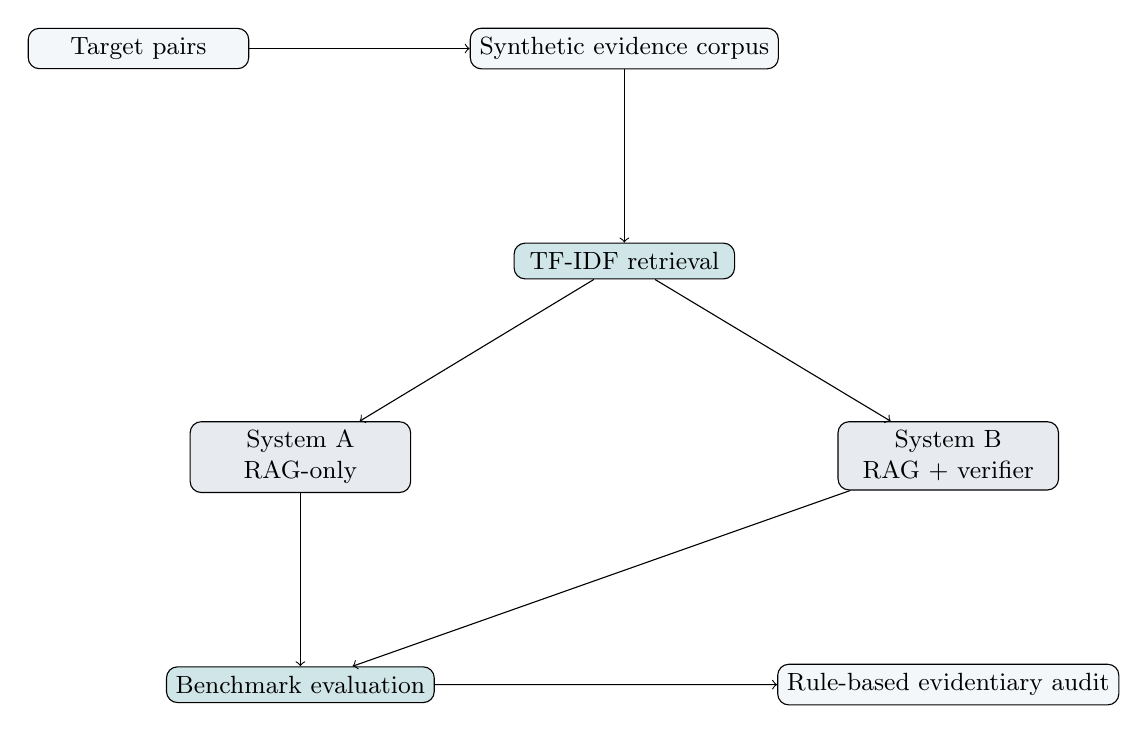
\begin{tikzpicture}[node distance=2.2cm and 2.8cm, every node/.style={font=\small}]
  \node[draw, rounded corners, fill=softgray, minimum width=2.8cm] (targets) {Target pairs};
  \node[draw, rounded corners, fill=softgray, minimum width=3.2cm, right=of targets] (corpus) {Synthetic evidence corpus};
  \node[draw, rounded corners, fill=teal!20, minimum width=2.8cm, below=of corpus] (retriever) {TF-IDF retrieval};
  \node[draw, rounded corners, fill=navy!10, minimum width=2.8cm, below left=1.8cm and 1.3cm of retriever] (a) {\shortstack{System A\\RAG-only}};
  \node[draw, rounded corners, fill=navy!10, minimum width=2.8cm, below right=1.8cm and 1.3cm of retriever] (b) {\shortstack{System B\\RAG + verifier}};
  \node[draw, rounded corners, fill=teal!20, minimum width=3cm, below=of a] (eval) {Benchmark evaluation};
  \node[draw, rounded corners, fill=softgray, minimum width=3cm, below=of b] (audit) {Rule-based evidentiary audit};

  \draw[->] (targets) -- (corpus);
  \draw[->] (corpus) -- (retriever);
  \draw[->] (retriever) -- (a);
  \draw[->] (retriever) -- (b);
  \draw[->] (a) -- (eval);
  \draw[->] (b) -- (eval);
  \draw[->] (eval) -- (audit);
\end{tikzpicture}
\caption{Actual pipeline implemented in the repository.}
\end{figure}

The code confirms the following implementation specifics:

\begin{itemize}[leftmargin=1.5em]
  \item \texttt{phase2\_retrieval/retriever.py}: deterministic TF-IDF + cosine-similarity retrieval over \texttt{phase2\_corpus/test\_retrieval\_documents.jsonl}.
  \item \texttt{phase2\_experiment/system\_a.py}: naive RAG heuristic; any co-occurrence or communication in retrieved documents can trigger a positive decision.
  \item \texttt{phase2\_experiment/system\_b.py}: identical retrieval budget, followed by formal verification through \texttt{phase2\_verification/verifier.py}.
  \item \texttt{phase2\_experiment/evaluator.py}: computes confusion metrics, McNemar statistics, and evidentiary soundness.
  \item \texttt{phase2\_ground\_truth\_vault/README.md}: formal quarantine and leakage-prevention guidance for the benchmark labels.
\end{itemize}

\section{Dataset and Benchmark Readiness}

The repository makes a clear distinction between public synthetic assets and the excluded raw upstream graph.

\begin{itemize}[leftmargin=1.5em]
  \item \textbf{Included public benchmark assets}: target pairs, sanitized evidence corpus, frozen outputs, run manifests, split manifest, and ground-truth vault metadata.
  \item \textbf{Excluded upstream source}: \texttt{israel\_lea\_inp\_burglary\_offender\_id\_network\_from\_2020-01-01\_to\_2020-06-30.json}, which is not in the repository because redistribution permissions are not verified.
  \item \textbf{Benchmark reproducibility}: the project is designed to evaluate on the sanitized synthetic corpus and frozen benchmark without the raw source network. The tests that require the raw dataset are explicitly skipped when the source is absent.
\end{itemize}

The benchmark readiness findings are:

\begin{itemize}[leftmargin=1.5em]
  \item 10-case pilot generated and present.
  \item 200-case test benchmark present and frozen.
  \item Target pairs, ground truth, manifests, evidence documents, provenance, and predictions are present.
  \item The benchmark split is isolated and leakage safeguards are enforced in tests.
  \item The raw source graph is not required for normal evaluation in the public repository.
\end{itemize}

\section{Implementation Inventory and Evidence Sources}

The actual experiment is built from the following code and data layers:

\begin{itemize}[leftmargin=1.5em]
  \item \texttt{phase2\_corpus/}: generated synthetic evidence corpus and public retrieval documents.
  \item \texttt{phase2\_retrieval/}: retrieval schema and TF-IDF indexing logic.
  \item \texttt{phase2\_verification/}: verifier and evidence-classification rules.
  \item \texttt{phase2\_experiment/}: runner, evaluator, System A/B implementations.
  \item \texttt{phase2\_ground\_truth\_vault/}: quarantined ground truth, pilot manifest, split manifest, and schemas.
  \item \texttt{docs/FINAL\_ACADEMIC\_REPORT.md}: final academic narrative and benchmark summary.
\end{itemize}

\section{Test-Suite Results}

The current environment was validated with the project test suite:

\begin{table}[h]
\centering
\begin{tabular}{l r}
\toprule
Metric & Value \\
\midrule
Passed & 148 \\
Failed & 0 \\
Skipped & 4 \\
Total & 152 \\
\bottomrule
\end{tabular}
\caption{Pytest execution summary from the current repository state.}
\end{table}

The skipped tests are expected and tied to the absent upstream dataset required for raw benchmark regeneration, not to repository corruption.

\section{Historical Baseline}

The metrics below were read from the frozen scoring report at \texttt{phase2\_experiment/outputs/full\_test\_scoring\_report.json}; they were not independently recalculated during this pre-push audit. They match the repository's documented claims:

\begin{table}[h]
\centering
\begin{tabular}{l rr}
\toprule
Metric & System A & System B \\
\midrule
Accuracy & 0.7000 & 0.7000 \\
Precision & 0.6250 & 1.0000 \\
Recall & 1.0000 & 0.4000 \\
Specificity & 0.4000 & 1.0000 \\
F1 score & 0.7692 & 0.5714 \\
False-positive rate & 0.6000 & 0.0000 \\
Evidentiary soundness & 0.1125 & 1.0000 \\
\bottomrule
\end{tabular}
\caption{Verified benchmark comparison from the frozen scoring report.}
\end{table}

The confusion-matrix counts are also consistent with the canonical report:

\begin{itemize}[leftmargin=1.5em]
  \item System A: TP=100, FP=60, TN=40, FN=0.
  \item System B: TP=40, FP=0, TN=100, FN=60.
\end{itemize}

\section{System B False-Negative Audit}

The historical condition breakdown reports that every missed positive for System B occurs in the alias ambiguity, missing evidence, and mixed-difficulty conditions. This establishes where the false negatives are counted, but not why any individual case was missed.

\begin{table}[h]
\centering
\begin{tabular}{l r r}
\toprule
Condition & System B Recall & Cases \\
\midrule
clean\_evidence & 1.0000 & 40 \\
alias\_ambiguity & 0.0000 & 40 \\
missing\_evidence & 0.0000 & 40 \\
distractors & 1.0000 & 40 \\
mixed\_difficulty & 0.0000 & 40 \\
\bottomrule
\end{tabular}
\caption{Historical System B recall by condition; condition labels do not establish case-level causes.}
\end{table}

The stored aggregate report records 20 false negatives in each of those three conditions. It does not provide sufficient case-level analysis here to establish whether a given case failed because evidence was absent, not retrieved, fragmented, unresolved, or rejected by verifier logic. Accordingly, no per-case root cause is confirmed in this report.

\section{Implementation Characteristics and Diagnostic Limits}

Code inspection establishes the following implementation characteristics. They are candidate mechanisms for future case-level investigation, not confirmed causes of the 60 false negatives.

\begin{itemize}[leftmargin=1.5em]
  \item \textbf{Single-pass retrieval}: the configured run uses top-5 lexical retrieval and does not enable re-retrieval. This does not show whether retrieval failed for a specific false-negative case.
  \item \textbf{Strict evidence gate}: the verifier requires qualifying solved-burglary evidence. A specific case's output and retrieved documents must be inspected before attributing its abstention to this rule.
  \item \textbf{Alias and contradiction handling}: aliases and contradictions are evaluated by deterministic verifier rules; their involvement in any particular false negative remains unverified here.
\end{itemize}

The most informative measured counts are:

\begin{itemize}[leftmargin=1.5em]
  \item System B false negatives: \textbf{60}. These occur in alias ambiguity (20), missing evidence (20), and mixed difficulty (20).
  \item System A unsound positives: \textbf{142} of 160 positive predictions were not supported by qualifying evidence.
  \item System A's unsound positives include 82 CDR-only cases and 60 insufficient-evidence cases.
\end{itemize}

The aggregate results show a precision/recall trade-off. They do not by themselves establish the case-level reasons for System B's false negatives.

\section{Most Promising Improvement}

The strongest improvement is not a blanket reduction in the verification threshold. Instead, the best next step is to address the retrieval bottleneck while preserving the verifier's evidentiary gate.

The repository already suggests the most promising direction:

\begin{itemize}[leftmargin=1.5em]
  \item Re-query or expand the evidence set when alias ambiguity or missing evidence is detected.
  \item Add explicit \texttt{Insufficient Evidence} versus \texttt{Evidence Against Relationship} states.
  \item Improve alias-resolution and entity-normalization before final rejection.
  \item Keep the verification threshold high enough to preserve the 0\% false-positive rate while recovering more legitimate positives.
\end{itemize}

This is a research direction, not a result established by the current aggregate audit. A case-level evidence trace review should precede any root-cause claim or system change.

\section{Controlled Next-Experiment Design}

The benchmark should remain frozen for final evaluation. Proposed next-step design:

\begin{enumerate}[leftmargin=1.5em]
  \item Baseline System A (unchanged).
  \item Baseline System B (unchanged).
  \item Improved System B variant with alias-aware re-retrieval or explicit evidence expansion.
  \item Separate development subset for tuning if valid new cases are available.
  \item Final comparison only on the frozen test set.
\end{enumerate}

The acceptance criteria should be proposed as research thresholds, not achieved results: recall improvement target, minimum soundness floor, and false-positive ceiling requiring owner approval before official adoption.

\section{Reproducibility and Integrity Audit}

The repository shows strong integrity controls. The actual benchmark file hash was checked and matched the manifest:

\begin{verbatim}
phase2_experiment/test_target_pairs.json
SHA-256: 125e012b794440c6db8170bb4aa9c385472780bddc1174c6ba7e76096c711cd0
Manifest match: True
\end{verbatim}

All tracked benchmark files in the private artifact manifest also matched their recorded hashes, and the public manifest matched as well. No benchmark input file was modified during this audit. No commit or push was performed.

\section{Data Governance and Scope Constraints}

The project documentation correctly states the main governance boundary: the raw upstream police network is excluded because redistribution permission is unverified. This is not a benchmark defect; it is a compliance and data-rights control. The repository therefore evaluates on a sanitized, public, deterministic corpus and does not claim to reproduce all upstream raw data in Git.

\section{Risks, Limitations, and Unresolved Questions}

\begin{itemize}[leftmargin=1.5em]
  \item Real-world external validity remains limited because the benchmark is synthetic and evidence-grounded rather than raw field operations.
  \item The verifier is conservative and may abstain even when some evidence is present but not fully resolved.
  \item The current repository does not provide a general live deployment path or field-ready monitoring system.
\end{itemize}

The strongest unresolved issue is the lack of a validated re-retrieval strategy that preserves high evidentiary standards without degrading recall too sharply.

\section{Prioritized Action Plan}

\begin{enumerate}[leftmargin=1.5em]
  \item Audit and instrument alias resolution pathways in the retrieval and verification stack.
  \item Add an explicit re-retrieval or expansion step for low-confidence ambiguous cases.
  \item Report \texttt{Insufficient Evidence} separately from \texttt{Evidence Against Relationship}.
  \item Keep the benchmark frozen and evaluate all improvements only on the untouched test set.
  \item Publish a next-phase report with per-condition metrics and a controlled comparison design.
\end{enumerate}

\appendix

\section{Appendix A: Commands and Observations}

This report was generated from repository inspection, hash verification, and live test execution on October 28, 2026. The following command outputs were observed:

\begin{verbatim}
python -m pytest phase2_corpus/tests phase2_retrieval/tests phase2_verification/tests phase2_experiment/tests phase2_ground_truth_vault/tests -v
Exit code: 0; 148 passed, 4 skipped, 0 failed (11.32s)
All four skips require the excluded raw Israel National Police source dataset.
\end{verbatim}

\begin{verbatim}
SHA-256 and artifact-manifest verification
phase2_experiment/test_target_pairs.json: MATCH
phase2_artifact_hash_manifest.json: 15/15 entries match
phase2_public_artifact_hash_manifest.json: 6/6 entries match
Total: 21 entries verified, 0 mismatches
\end{verbatim}

\section{Appendix B: PDF Compilation}

The report was compiled successfully with MiKTeX 25.12 using \texttt{pdflatex}. The resulting PDF is included alongside this source as \texttt{research\_audit/SPYDER\_Research\_Audit\_and\_Next\_Phase.pdf}.

\begin{verbatim}
pdflatex -interaction=nonstopmode -halt-on-error SPYDER_Research_Audit_and_Next_Phase.tex
Exit code: 0
\end{verbatim}

\end{document}
